\section{Sarrera.}

\subsection{Context of the Study}

Urte luzez, zientzia arlo ezberdinek N-gorputzeko problema ikertu dute. Arlo nagusien artean aipatu daiteke, astronomoek Eguzki-Sistemaren planeten mugimendua ulertu nahian egidako lana edo kimikariek erreakzio kimikoekin esperimentatzeko molekulen dinamikaren azteketa. Arlo bakoitzak bere ezberditasunak (adibidez lege fisikoak) baditu ere, oinarrian problema berdina lantzen dutenez hauen arteko antzekotasun handiak daude. Azpimarratu ere,  N-gorputzen problemaren azterketak garrantzi berezia izan duela matematikako eremu ezberdinen garapenean, esaterako dinamika ez-lineal eta kaos teorian. 

Garai batean, N-gorputzen problemen azterteketak teori analitikoen bidez egiten ziren baina konputagailuen sorrerarekin, zenbakizko integrazioak bilakatu ziren tresna nagusia. Urteekin, bai konputazio teknologien aurrerapenari bai algoritmo berrien sorrerari esker, zenbakizko azteketek garapen handia izan dute. Zenbakizko simulazioen laguntzaz, Eguzki-Sistemaren mugimenduaren funtsezko galdera batzuk ezagutu ditugu eta berriki, Karplusen taldeak 2013. kimikako nobel saria jaso du kimika konputazionalean egindako lanarengatik.       

Guk lan honetan, N-gorputzen problema grabitazionala aztertuko dugu. Orohar eta gaia kokatzeko asmoarekin, N-gorputzen zenbakizko ohiko integrazioak hiru taldeetan sailkatu ditzakegu:
\begin{enumerate}
{
\item Epe motzeko eta doitasun oso handiko integrazioak. 
 Eguzki-Sistemaren efemeride zehatzak edo espazioko satelite artifizialen kokapenen kalkuluetarako erabili ohi dira.
\item Epe luzeko integrazioak baina doitasun handi gabekoa.
 Denbora oso luzean planeta-sistemen mugimendu ezagutzeko egindako ikerketak ditugu. Azterketa hauetan, garrantzitsua da gorputzen mugimenduaren  argazkia orokorra ezagutzea baina zehaztasun handirik gabe. Normalean gorputzen arteko kolisio gertuko egoerak egoerak ez dira agertzen.     
\item N-gorputz kopurua edozein izanik, hauen arteko kolisioak gerta daitezkeen problemak.
 Integrazio hauetan, konplexutasun handiari aurre egin behar zaio : N-gorputz kopurua miliotako izan dateke; gainera kolisio gertuko egoeren ondorioz, kalkulutan egindako zenbakizko errore txikiek eragin handia izan ditzakete soluzioan.
    
}
\end{enumerate}

Gure lana goian sailkatutako integrazio moten nahasketa da, gure helburua Eguzki-Sistemaren epe luzeko eta doitasun handikoa algoritmoak garatzea baita. Aurreko hamarkadetan, Eguzki-Sistemaren planeten epe luzeko zenbakizko integrazioa erronka garrantzitsua izan zen. Adibidez, Sussmanek eta Wisdomek (1993) Eguzki sistemaren 100 miliotako integrazioaren bidez, planeten mugimendua kaotikoa zela baieztatu zuten. Aldi berean, paleoklimatologia zientziak orain milioika urte gertatutako klima zikloak  azaltzeko (epel, hotz eta glaziazio artekoa), Lurraren orbitan izandako aldaketaren eraginez gertatu zela azaltzen duen teoria (Milankovitch 1941) frogatzeko planeten orbiten efemeride zehatzak beharrezkoak dira.        

Konputazio-teknologi arrerapenak handiak izan arren, Eguzki sistemaren simulazio hauek konputazionalki oso garestiak dira eta exekuzio denbora luzeak behar dituzte (Laskar La2010a 18 hilabete). Azken urteotako konputagailu berrien arkitekturaren bilakaerak, algoritmo azkarren diseinua aldatu du: simulazioak azkartzeko paralelizazioan oinarritu behar dira eta eragiketa aritmetikoek baino kostu handiagoa du memorien arteko datu komunikazioak. Beraz, oraindik ere algoritmo eraginkorragoak beharrezkoak dira eta gaur egun hauek garatzeko bide berriak ikertu behar dira.


\subsection{Problem statement or motivation for the study.}
\label{intro}

Gaur egun, epe luzeko integrazioetarako hainbat zenbakizko metodo erabiltzen dira bereziki beren izaera Hamiltondarra mantentzen duten metodoak (metodo sinpletikoak). Metodo horien artean, gehien erabiltzen direnak izaera esplizituko algoritmoak dira.

Lehenik, metodo esplizitu eta inplizituei buruz dagoen ikuspegi nagusia aipatu nahi genuke. Metodo esplizituak problema ez-stiffa denean metodo inplizituak bainon eraginkorragoak dira. Metodo inplizituek duten eraginkortasun arazo handiena ekuazio sistema ez-lineala askatzea da, eta honek metodo esplituekiko CPU denbora gainkarga suposatzen du. Horregaitik problema ez-stiffa bada, metodo esplizituak erabili ohi dira eta problema stiff-a denean bakarrik jotzen dugu metodo inplizituengana. Baieztapen hau eztabaidagarria da, eta praktikan metodo inplizituetan gehiago sakondu behar dela iruditzen zaigu. 

Euler metodo esplizitua.					  
\begin{equation}
y_{n+1}=y_n+hf(y_n)
\end{equation}

Euler metodo inplizitua.
\begin{equation}
y_{n+1}=y_n+hf(y_{n+1})
\end{equation}

Zentzu honetan, metodo inplizituen ezaugarri interesgarri batzuk nabarmenduko ditugu. Abantaila nagusienetakoa malgutasuna da.  Metodo inplizituek inplementazio malgua onartzen dute eta ondorioz, integratu nahi dugun problemari egokitzeko aukera gehiago eskeintzen dizkigu. Aipatzekoa da ere, metodo esplizituak sistema Hamiltondar banagarrietan bakarrik aplika daitezkeela: Hamiltondarraren egitura hau aprobetxatuz oso eraginkorrak dira baina integratu nahi den problemak bete behar duen muga ere. Metodo inplizituak aldiz, Hamiltondar orokorrei aplika daitezke eta gainera, lehen ordenako ekuazio diferentzialetarako  metodo sinpletikoak inplizituak izan behar dira.  Azkenik ez dugu ahaztu behar, metodo inplizituen artean orden altuko metodoak existitzen direla  eta hauek nahitaezkoak dira doitasun handiko integrazioak behar ditugunean.     

Lan honetan, metodo inplizituen artean Gauss zenbakizko integrazio metodoa aukeratu dugu. Hainbat autorek (Hairer eta Sanz Serna) metodo honen potentziala nabarmendu dute eta guk ere, iritzi berekoak gara. Laburki aipatuz, $s$ ataletako metodo hau $2s$ ordenekoa da, sinpletikoa da, estabilite ezaugarri onak ditu eta paralizatzeko gaitasuna ahaztu gabe.      

\subsection{Aim and scope}

Gure helburua, Eguzki Sistemaren ebazpenerako Gauss inplizituaren inplementazio eraginkorra proposatzea da. Hau lortzeko  bereziki honako aspektu hauek kontutan izango ditugu: Eguzki-sistemaren problemaren ezaugarriak, konputagailuen koma-higikorreko aritmetika eta algoritmo paraleloen abantaila.  

N gorputzeko problema grabitazionalari dagokionez, Eguzki sistemaren eredu sinplea integratuko dugu. Eguzki sistemaren gorputzak masa puntualak kontsideratuko ditugu eta gure ekuazio diferentzialek, gorputz hauen arteko erakarpen grabitazionalak bakarrik kontutan hartzen dituzte. Beraz, eguzki sistemaren eredu konplexuagoetako erlatibitate efektua, gorputzen formaren eragina, eta beste zenbait indar ez-grabitazionalak ez dira kontutan hartu.
Bestalde era honetako integrazioetan, gorputzen hasierako balio eta parametro zehatzak sateliteen bidez jasotako datu errealekin bat datoztela egiaztatze prozesua ez dugu landu.

Zeintzuk dira Eguzki-sistemaren problemaren ezaugarri bereziak? Batetik bi gorputzen problemaren (kepler problema) soluzioa zehatza ezaguna da eta Eguzki-Sistemaren gorputzen mugimenduaren konputazioaren oinarria. Bestetik,  badugu gorputz nagusi bat (Eguzkia) eta honen inguruan bueltaka sailkatutako planetak: barne planetak, masa txikikoak eta eguzkitik gertu daudenak ; kanpo planetak, masa handikoak eta eguzkitik urrun daudenak (ikus irudia Fig.\ref{fig:plot1}). Eguzki-Sistemaren egitura honi abantaila handien lortzen duen planteamendua bilatuko dugu.



\begin{figure}[h]
\centering
\subfloat[Planeten arteko distantziak.]{
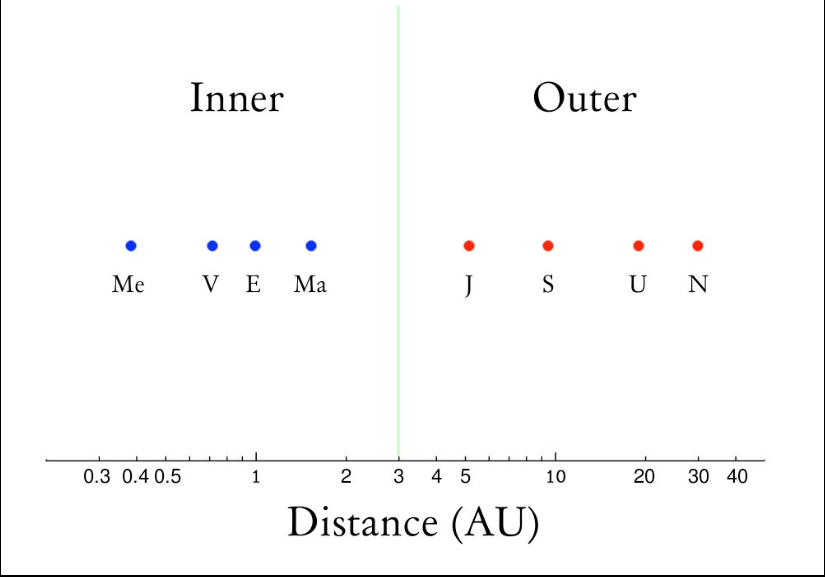
\includegraphics[width=.500\textwidth]{eguzkisistema1}
}
\subfloat[Planeten arteko masa konparaketa.]{
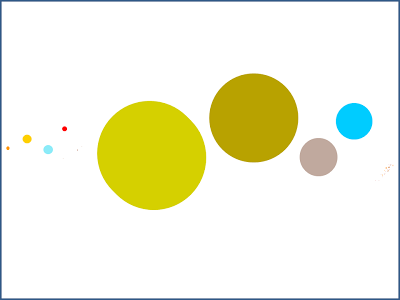
\includegraphics[width=.500\textwidth]{eguzkisistema2}
}
\caption{\small Eguzki-sistema.}
\label{fig:plot1}
\end{figure}    
   
Konputagailuen koma-higikorreko aritmetika ondo ulertzea garrantzitsua da. Zenbaki errealen adierazpen finkoa erabiltzen denez bai zenbakiak memorian gordetzeko, bai hauen arteko kalkulu aritmetikoak egiteko, errore bat egiten dugu. Integrazio luzeetan errore hau propagatzen da eta une batetik aurrera, soluzioen zuzentasuna ezereztatzen da. Ondorioz, integrazioan zehar errore honen monitorizazioa ezagutzea interesgarria da eta integrazio luzeen kasuan, doitasun handian lan egiteko beharra azaltzen zaigu. Gaur egun doitasun altuko aritmetiken erabilera oso garestia da, inplementazioa software bidezkoa delako. Exekuzio denborak onargarriak lortzeko tarteko irtenbidea, inplementazioan doitasun ezberdinak nahastea izango litzateke.       

Sarrera honetan paralelizazioari buruzko ohar bat ematea komeni da. Algoritmo baten kode unitateak paraleloan exekutatzeak badu gainkarga bat eta beraz,  algoritmoaren exekuzioa paralelizazioaz azkartzea lortzeko,  unitate bakoitzaren tamainak esanguratsua izan behar du. Gure Eguzki-sistemaren eredua sinplea da eta logikoa da pentsatzea eredu konplexuagoetan, paralelizazioak abantaila handiagoa erakutsiko duela. Bestalde $N$ gorputzen kopurua handia den problemetan, hauen arteko interakzio kopuru $O(N^2)$ handia kalkulatu behar da eta indar hauen hurbilpena modu eraginkorrean kalkulatzeko metodo ezagunak daude: \textit {tree code} eta \textit {fast multipole method}. Baina gure probleman gorputz kopurua txikia denez, ideia hauek gure eremutik kanpo utzi ditugu. 

\subsection{Overview of the study (structure of the Thesis).}

Gure lanaren abiapuntua Hairer-en IRK metodoaren inplementazioa da. Autoreak IRK puntu-finkoaren inplementazio estandarrean biribiltze errorearen okerreko konportamenduaz jabetu zen eta arazo hau konpontzeko soluzioak proposatu zituen. Lehen urratsa honetan, biribiltze errorearen arazoari soluzio berri bat eman diogu eta gure IRK inplementazioaren oinarriak finkatu: formulazio, koefizienteak, geratze erizpidea,atalen hasierketa \dots.
Gure inplementazioak biribiltze errorea propagazioa optimotik gertu dagoela baieztatzeko, \textit {integratzaile idealaren} soluzioarekin konparatu dugu. Aldi berean, integratzailean biribiltze errorearen estimazioa monitorizatzeko aukera garatu dugu.

Bigarren urratsean, ekuazio sistema ez-lineala ebazteko puntu-finkoaren ordez, Newton sinplifikatuaren metodoa aztertu dugu. Gure ekarpena, Newton sinplifikatua modu eraginkorrean aplikatzeko teknika proposatzea izan da. S-ataletako IRK metodoa eta d-dimentsioko EDA baditugu, Newton sinplifikatuaren metodoren iterazio bakoitzean $sdxsd$ tamainako sistema linealak askatu behar dira. Gure proposamena da, jatorrizko sistema lineala blokeka diagonala den sistema baliokide gisa beridaztea eta matrizearen egitura hau aprobetxatu sistema modu eraginkorrean askatzeko.

Hirugarren urratsean, Eguzki-sitemaren epe luzeko integrazioan arituko gara. Ekarpen handiena, atalen hasieraketa berri bat aplikatzea da alde kepleriarraren fluxuan oinarrituz. IRK metodoak eskeintzen digun malgutasunari esker eta N gorputzetako problema grabitazionalaren ezaugarrietaz baliatuz inplementazio ezberdinak egingo ditugu. Inplementazio hauen eraginkortasuna, egungo integratzaile simplektiko esplizituekin konparatuko ditugu.

Azken urratsean, esperimentalki , eguzki-sistemaren integrazioan  birparametrizazio teknikaren aplikazio sinple bat erakutsiko dugu. Integratzaile sinpletikoak luzeera finkoko urratsa eduki behar du eta zentzu honetan,birparametrizazioa eraginkortasuna hobetzeko beste bide bat da.             
      
\subsection{laburpena}

